\section{Studies of jet properties}
\label{sec:jets}

We consider several variables that characterize jet substructure using different calorimeter granularities. The question we want to answer is, how closely the reconstructed
jet substructure variables reflect the input ``truth'' values  that are reconstructed using particles directly from the \pythia generator.

In this study we use the jet effective radius and jet splitting scales as benchmark variables
to study jet substructure properties \textcolor{red}{with the signal $Z'\rightarrow WW$ process only}. 
The effective radius is the average of the energy-weighted radial distance $\delta R_i$ in $\eta-\phi$ space of jet constituents.
It is defined as $(1/E) \sum_i e_i \delta R_i$, where $E$ is the energy of the jet and $e_i$ is the energy of a calorimeter 
constituent cluster $i$ at the distance $\delta R_i$ from the jet center. The sum runs over all constituents of the jet. 
This variable has been studied for multi-TeV jets in Ref.~\cite{Auerbach:2014xua}.
A jet $k_T$ splitting scale~\cite{Butterworth:2002tt} is defined as a distance measure
used to form jets by the $k_T$ recombination
algorithm~\cite{Catani1993187,Ellis:1993tq}.
This variable has been studied by ATLAS~\cite{ATLAS:2012am}, and more recently in the context of 100 TeV physics~\cite{Auerbach:2014xua}.
The splitting scale is defined as $\sqrt{d_{12}}=\min(p_T^1,p_T^2) \times \delta R_{12}$~\cite{ATLAS:2012am} 
 at the final stage of the $k_T$ clustering, where two subjets are merged into the final jet.

Figures~\ref{fig:eff_rad} and~\ref{fig:d12} show the distributions of 
the jet effective radius and jet splitting scale for  different jet transverse momenta and HCAL granularities. 
The reconstructed-level distributions  disagree significantly with the distributions  
reconstructed using truth-level particles. The distributions reconstructed with 1~$\times$~1~cm$^2$ or 5~$\times$~5~cm$^2$ cells 
 are generally closer to the truth-level variables, than the distributions 
reconstructed using 20~$\times$20~cm$^2$ cells, particularly for resonance masses in the 10-20 TeV range. In these cases, there is not much  difference between the 
 5~$\times$~5~cm$^2$ and  1~$\times$~1~cm$^2$ cell sizes. \textcolor{red}{The extreme case with $M(Z')=40$ TeV corresponds to very boosted jets, 
with roughly $p_T \simeq 20$~TeV for each jet.  This case does not show 
differences between different detector configurations.}

This study confirms the baseline SiFCC detector geometry~\cite{Chekanov:2016ppq} that uses $5 \times 5$~cm$^2$ HCAL cells,
corresponding to $\Delta \eta \times \Delta \phi = 0.022\times0.022$.
Similar HCAL cell sizes,  $0.025\times0.025$,  were recently adopted for the baseline FCC-hh detector~\cite{fcc1,fcc2} planned at CERN.
Before the publication~\cite{Chekanov:2016ppq},   such a choice for the HCAL cells   
was motivated by the studies of jet substructure  using a fast detector simulation of boosted jets.
In addition to the improvements in physics performance, the smaller HCAL cells 
reduce the required dynamic range for 
signal reconstruction~\cite{Chekanov:2015ihl}, and thus can simplify the calorimeter readout.

It should be noted that the ATLAS and CMS detectors use the HCAL cell sizes in the barrel region which are close to 
$\Delta \eta \times \Delta \phi = 0.087\times 0.087$. \textcolor{red}{Both experiments focus on jet substructure variables for jets with 
transverse momenta below 4~TeV.
Our studies indicate that the future experiments, which will measure 
jets with transverse momenta above this value, require a higher
granularity of HCAL cell sizes in order to achieve the most optimal 
performance for jet substructure variables.
In the following sections we consider several other physics-motivated
variables that can shed light on the performance of the HCAL for tens-of-TeV jets.}


\begin{figure}
\begin{center}
   \subfigure[$M(Z')=5$~TeV] {
   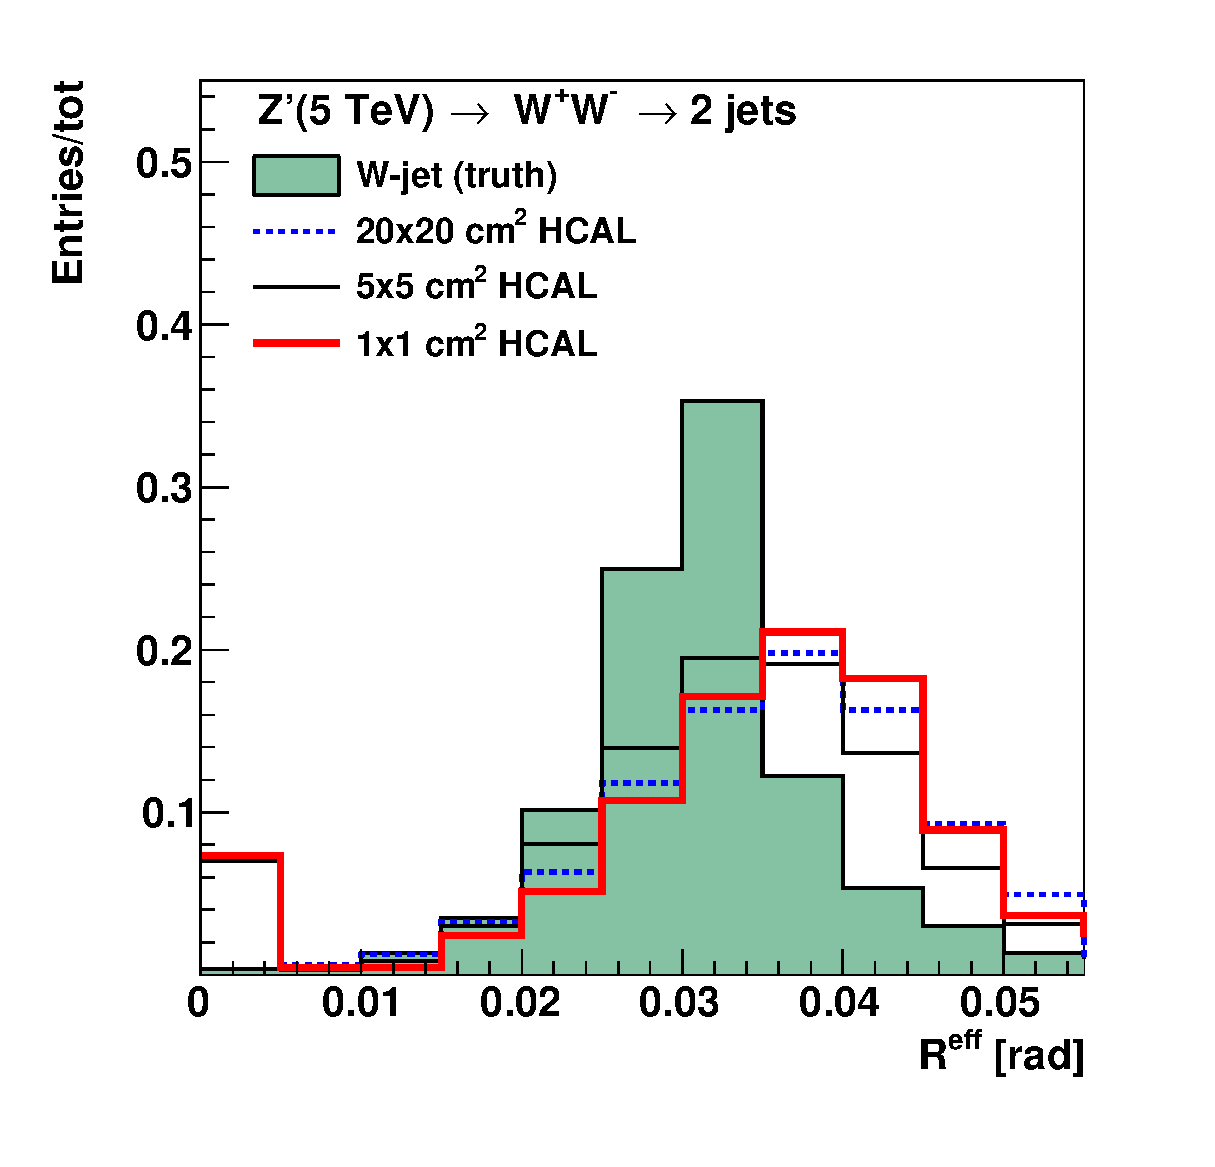
\includegraphics[width=0.46\textwidth]{figs/h5tev_clus_effR_ww1}\hfill
   }
   \subfigure[$M(Z')=10$~TeV] {
   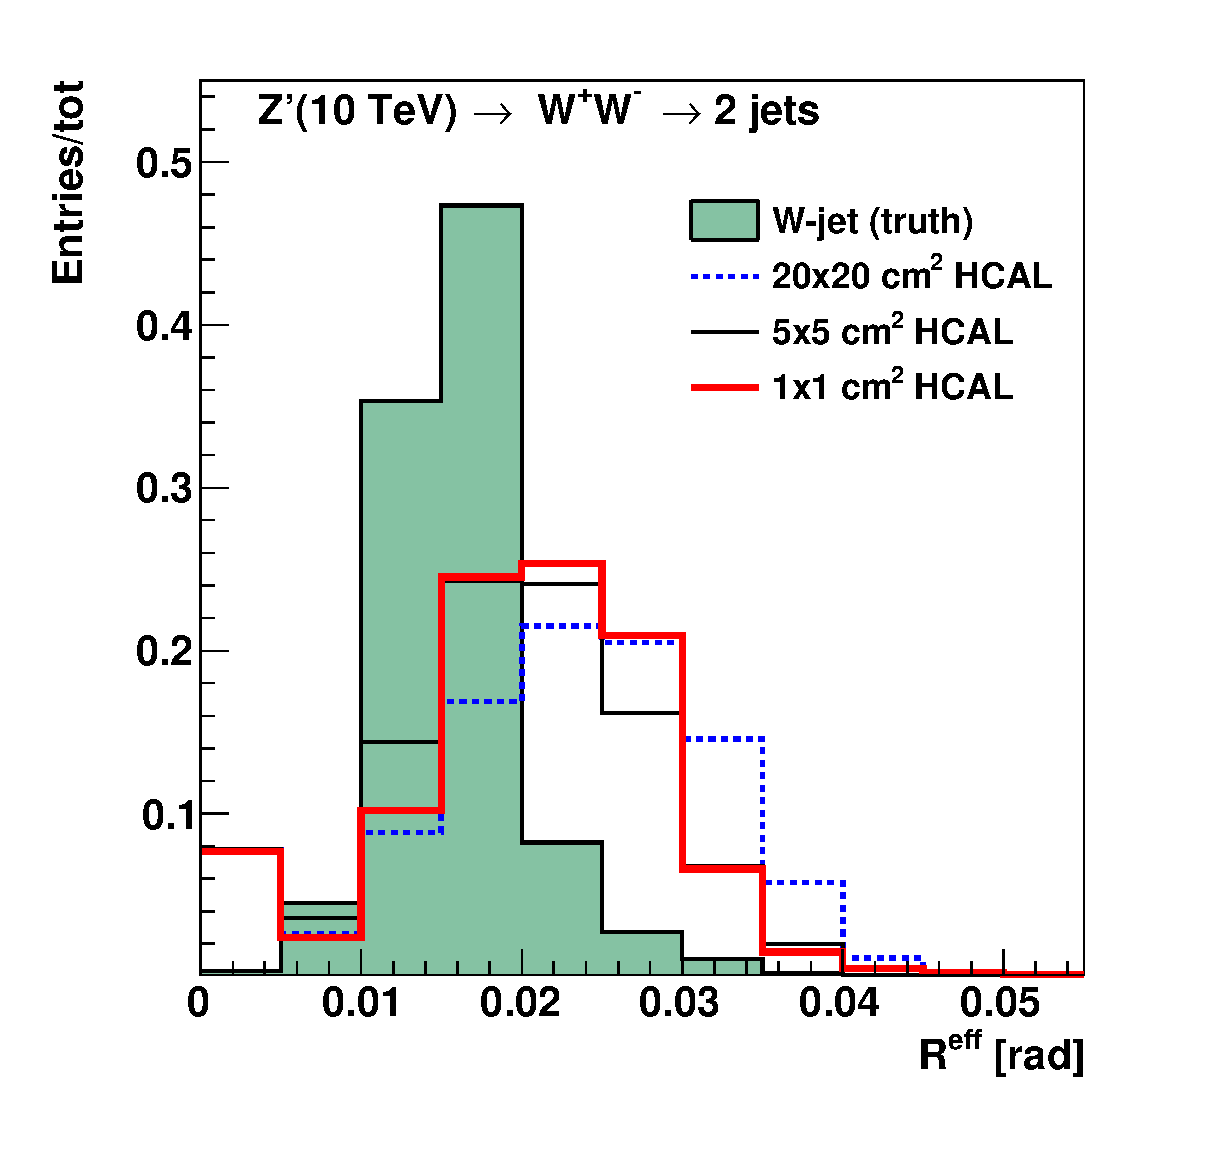
\includegraphics[width=0.46\textwidth]{figs/h10tev_clus_effR_ww1}
   }
   \subfigure[$M(Z')=20$~TeV] {
   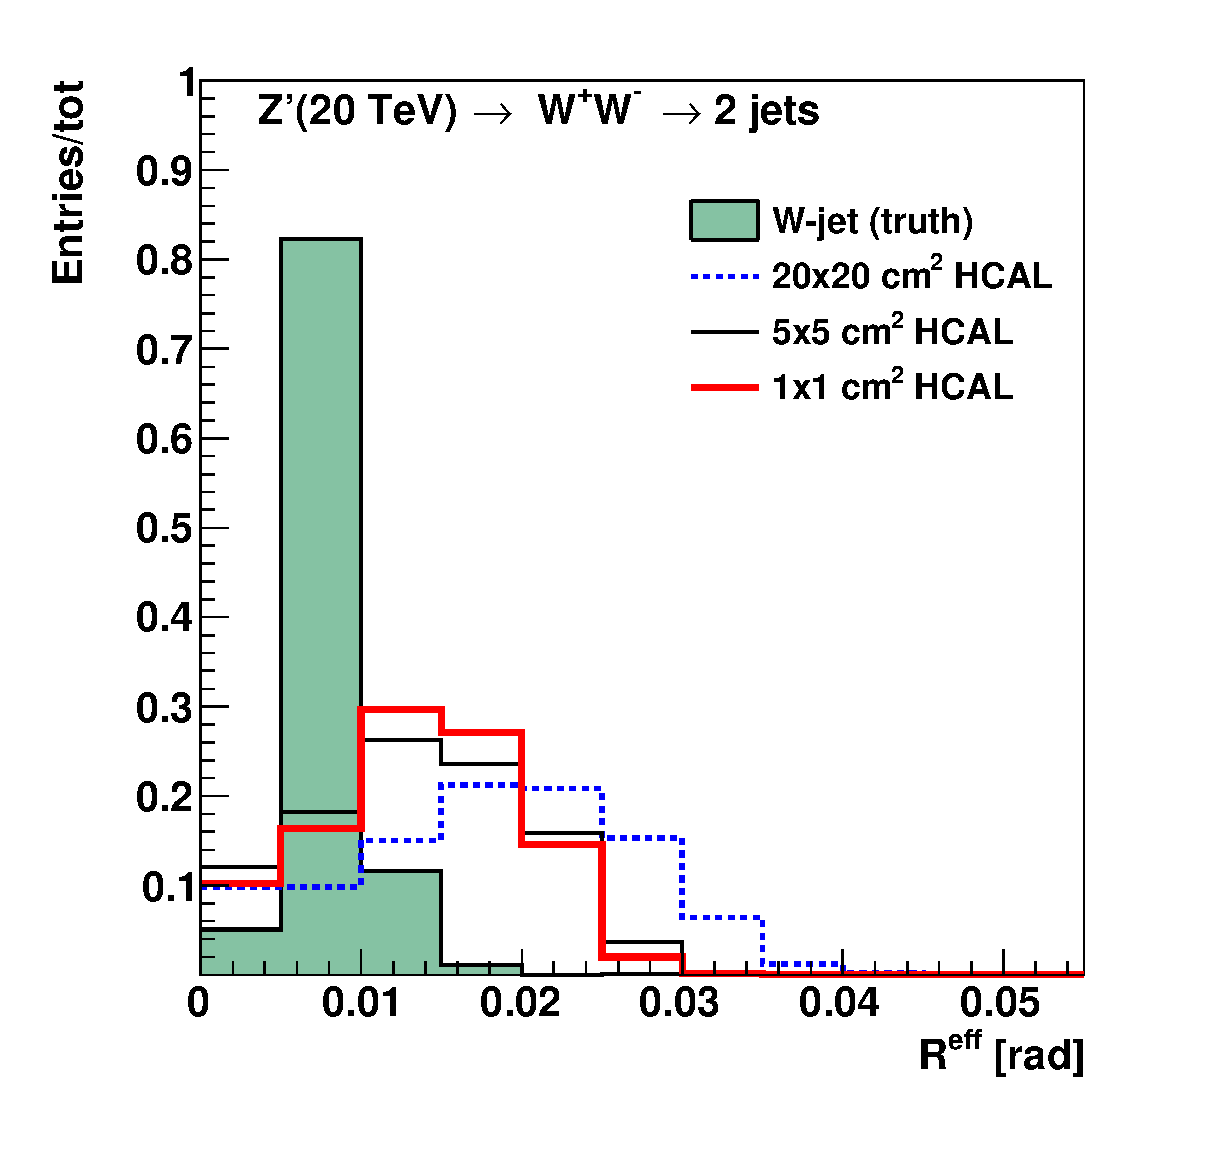
\includegraphics[width=0.46\textwidth]{figs/h20tev_clus_effR_ww1}
   }
   \subfigure[$M(Z')=40$~TeV] {
   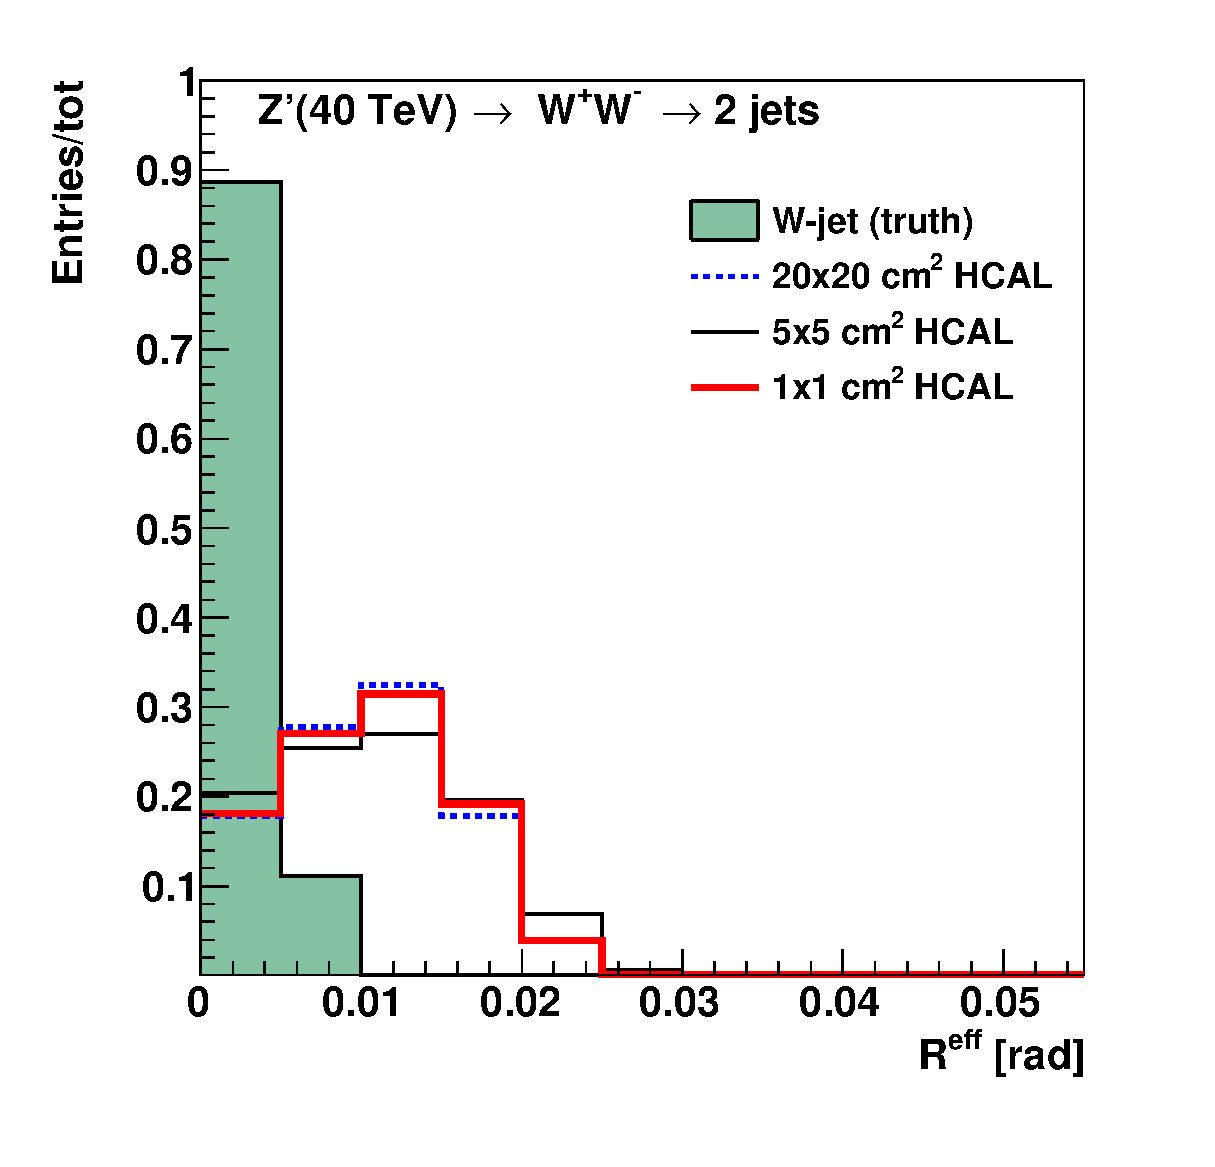
\includegraphics[width=0.46\textwidth]{figs/h40tev_clus_effR_ww1}
   }
\end{center}
\caption{Jet effective radius for different jet transverse momenta and HCAL granularities.}
\label{fig:eff_rad}
\end{figure}


\begin{figure}
\begin{center}
   \subfigure[$M(Z')=5$~TeV] {
   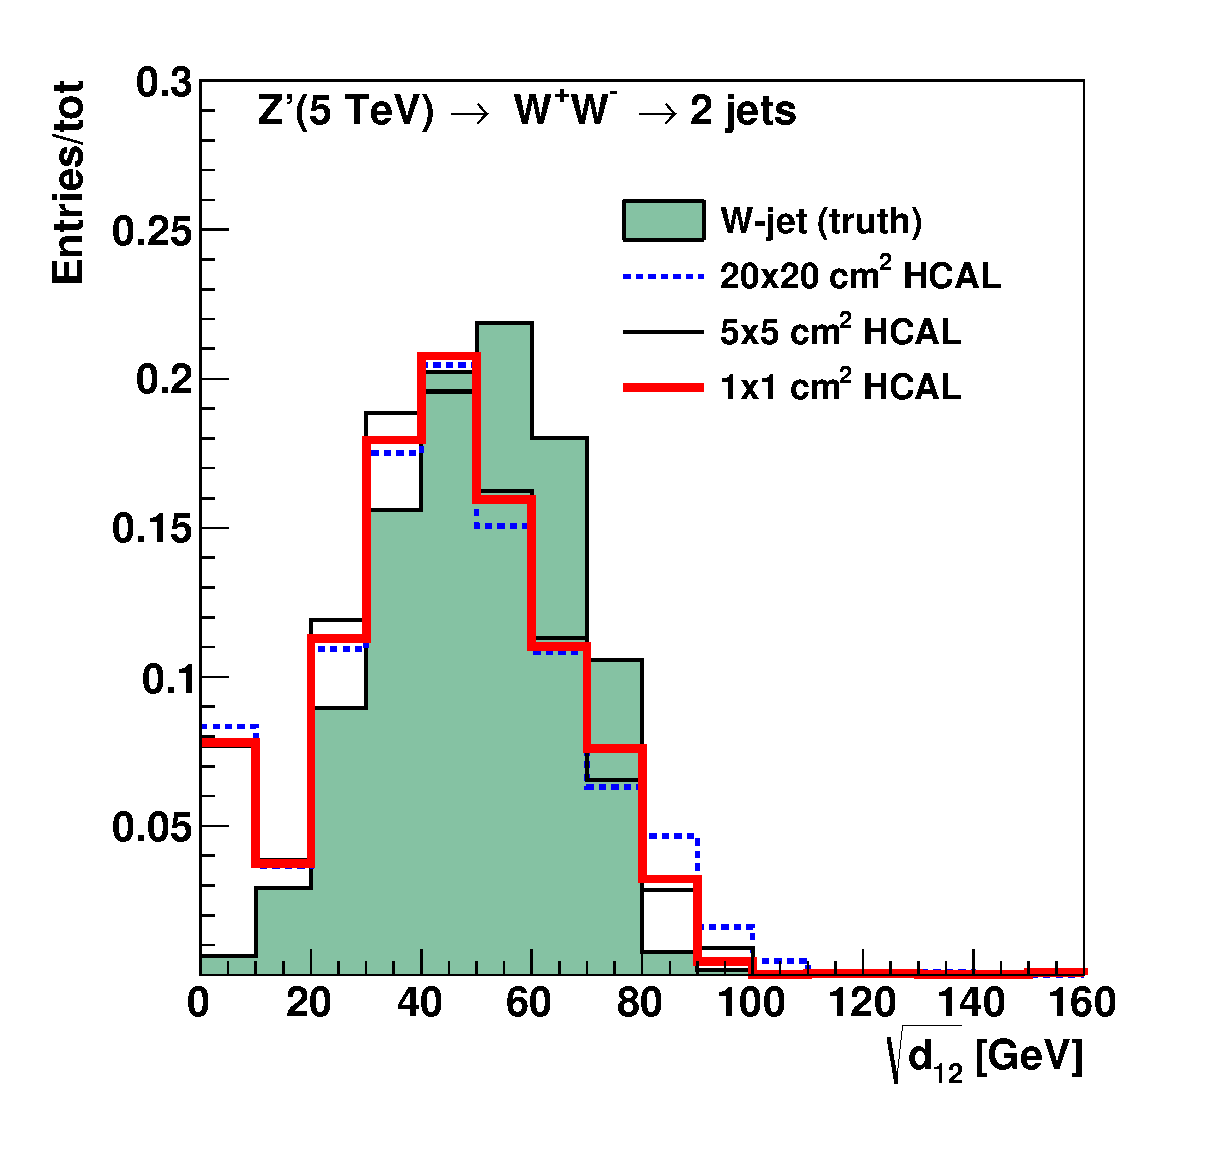
\includegraphics[width=0.46\textwidth]{figs/h5tev_clus_d12_ww1}\hfill
   }
   \subfigure[$M(Z')=10$~TeV] {
   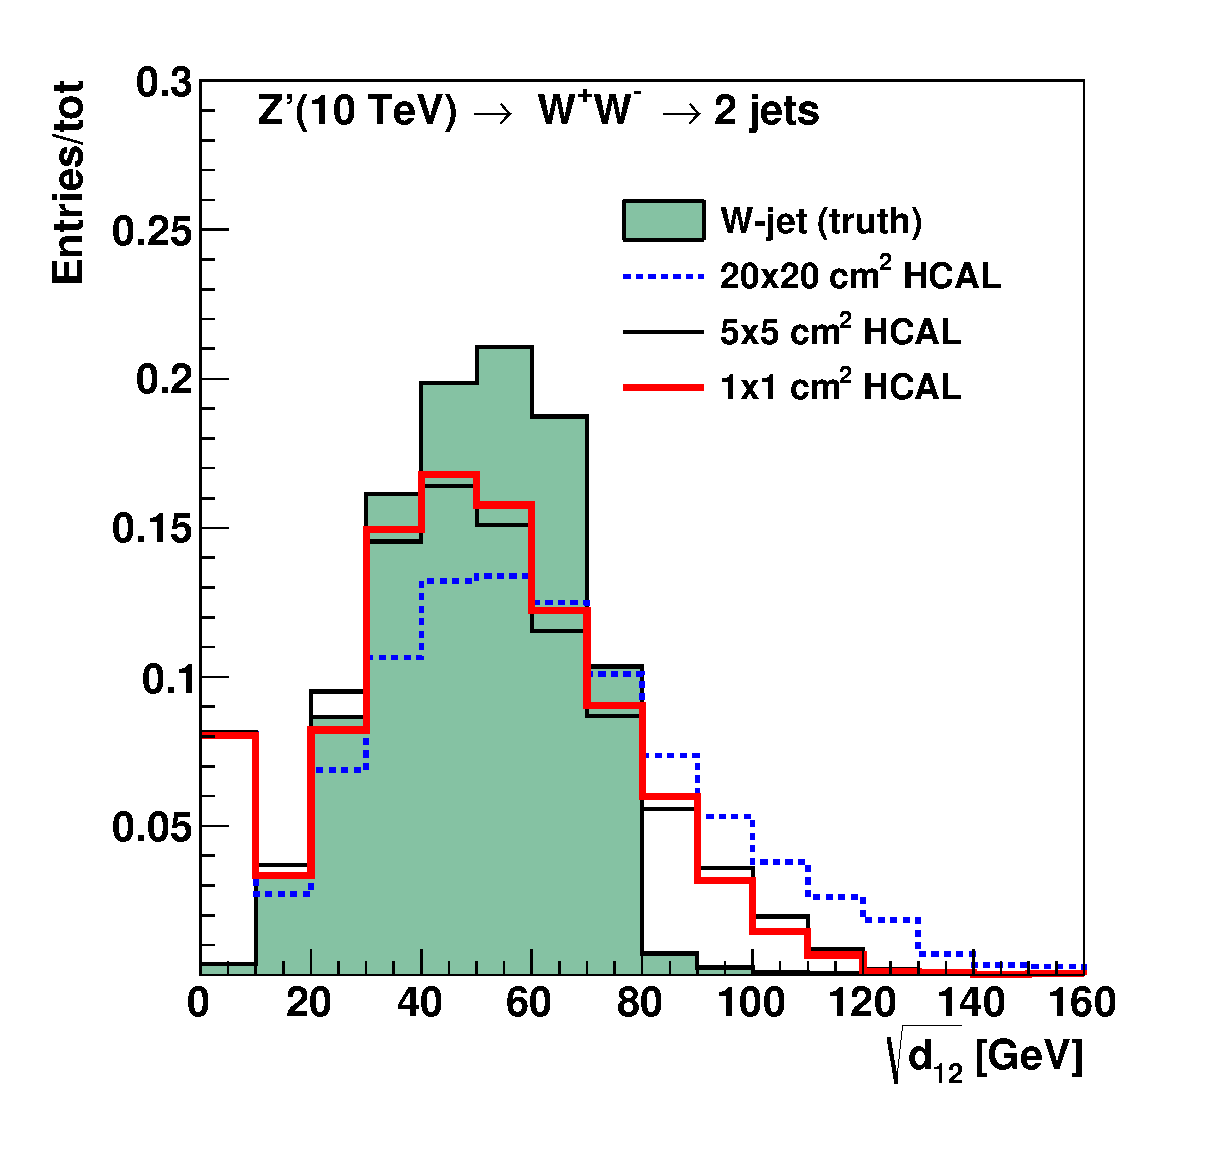
\includegraphics[width=0.46\textwidth]{figs/h10tev_clus_d12_ww1}
   }
   \subfigure[$M(Z')=20$~TeV] {
   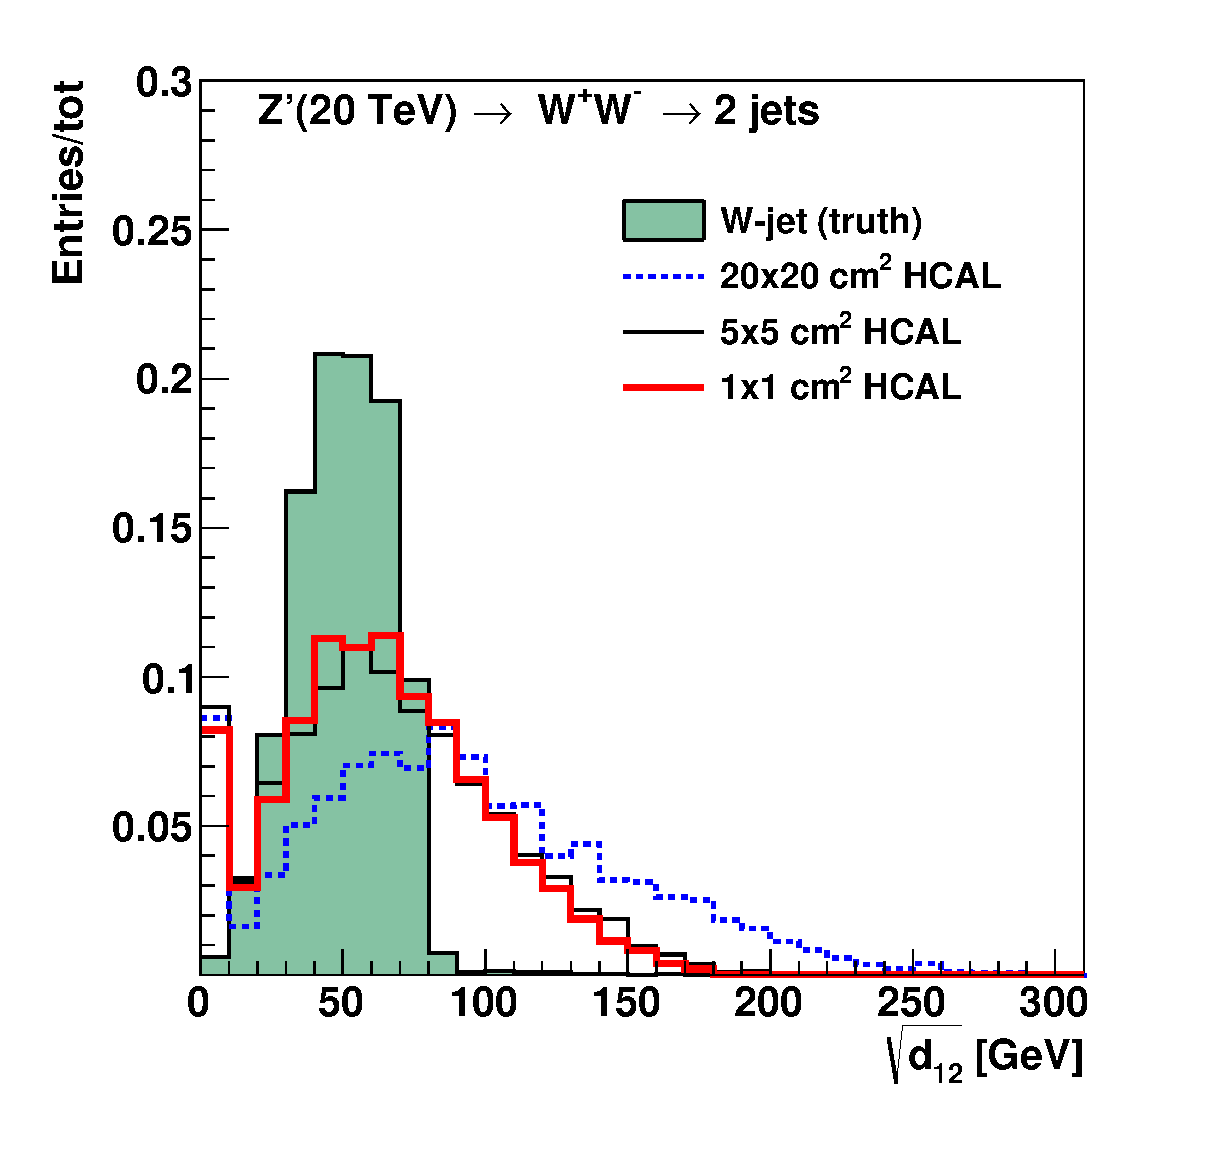
\includegraphics[width=0.46\textwidth]{figs/h20tev_clus_d12_ww1}
   }
   \subfigure[$M(Z')=40$~TeV] {
   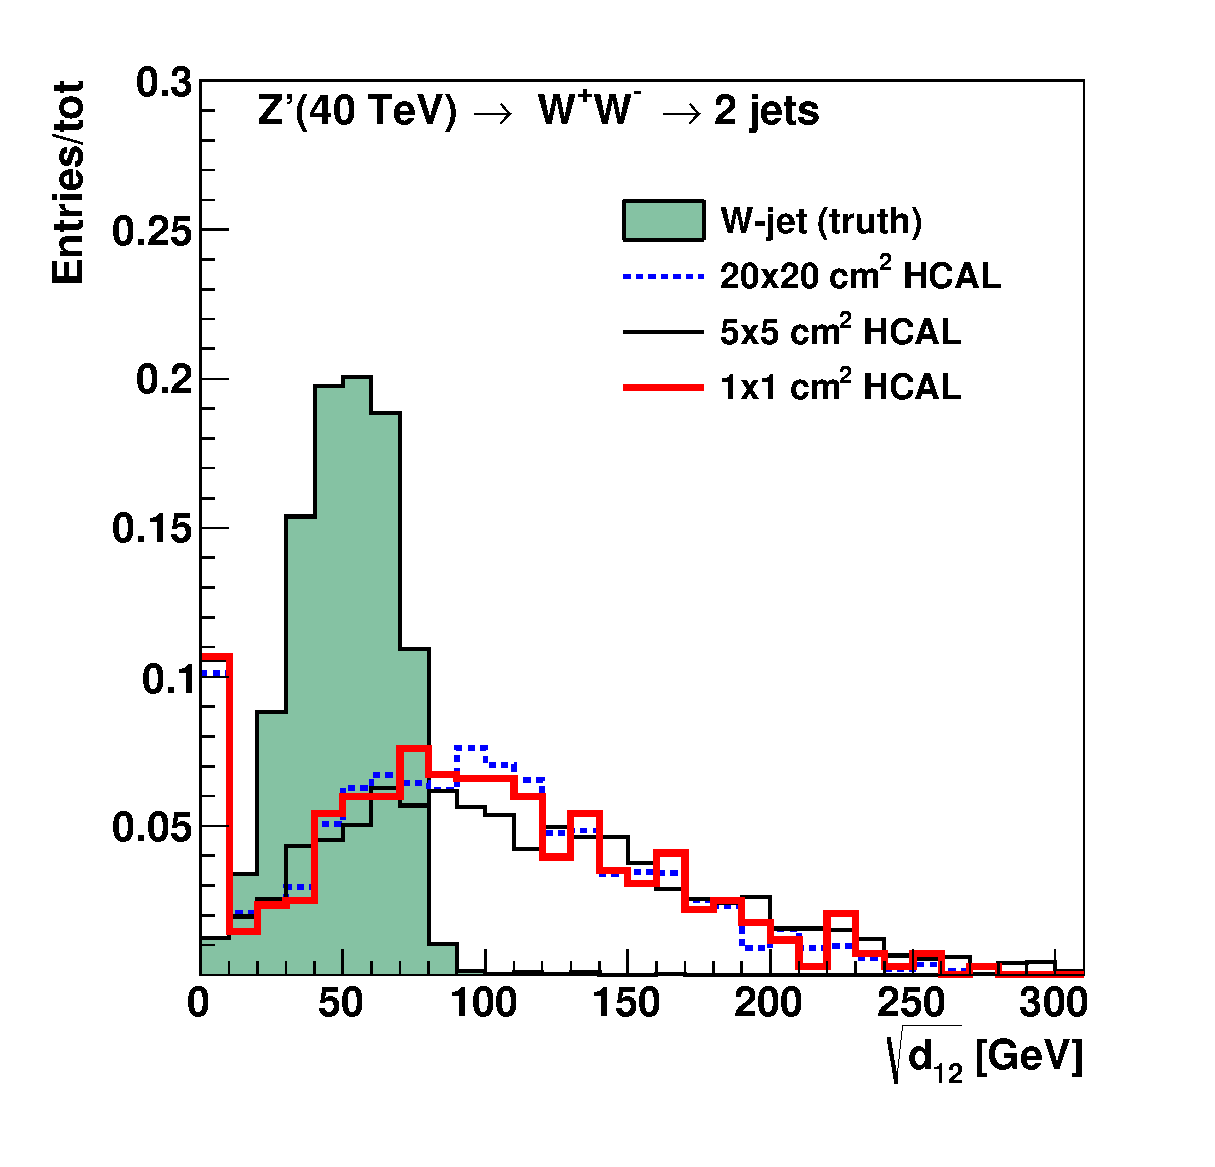
\includegraphics[width=0.46\textwidth]{figs/h40tev_clus_d12_ww1}
   }
\end{center}
\caption{Jet splitting scale for different jet transverse momenta and HCAL \textcolor{red}{granularities}.}
\label{fig:d12}
\end{figure}


%%%%%%%%%%%%%%% commented out 
\begin{comment}

\subsection{Jet subjettiness}

We recall that $N$-subjettiness~\cite{Thaler:2010tr}, $\tau_{N}$, of jets has been proposed
as a class of variables with which to study the decay products of a heavy particle inside jets.  $\tau_{N}$ is a measure of the degree to which a jet can be considered as being composed of
 $N$  $k_{T}$-subjets \cite{Thaler:2010tr}. 
The variable $\tau_{32}$, defined as the ratio of the $N$-subjettiness variables $\tau_3/\tau_2$, is particularly sensitive to hadronically-decaying
 top-quark initiated jets.
The variable, $\tau_{21} \equiv \tau_2/\tau_1$ can be used to reject background from $W/Z$ decays.
These variables do not strongly correlate with jet mass and can provide an independent check for the
presence of top quarks.
The jet substructure variables were obtained by re-running the $k_T$ algorithm over the jet constituents of anti-$k_T$ jets.

As an example of the effect of the calorimeter granularity, 
\begin{figure}
\begin{center}
   \subfigure[5 TeV] {
   \includegraphics[width=0.43\textwidth]{figs/r09_tau21b1_20tev_04_U.pdf}\hfill
   }
   \subfigure[10 TeV] {
   \includegraphics[width=0.43\textwidth]{figs/r010_tau21b1_20tev_04_U.pdf}
   }
   \subfigure[20 TeV] {
   \includegraphics[width=0.43\textwidth]{figs/r012_tau21b1_20tev_04_U.pdf}
   }
\end{center}
\caption{Jet subjetinness $\tau_{21}$ for jets originating from splitting scale for different jet transverse moment and HCAL granularity.}
\label{fig:tau21}
\end{figure}


\begin{figure}
\begin{center}
   \subfigure[5 TeV] {
   \includegraphics[width=0.43\textwidth]{figs/r09_tau32b1_20tev_04_U.pdf}\hfill
   }
   \subfigure[10 TeV] {
   \includegraphics[width=0.43\textwidth]{figs/r010_tau32b1_20tev_04_U.pdf}
   }
   \subfigure[20 TeV] {
   \includegraphics[width=0.43\textwidth]{figs/r012_tau32b1_20tev_04_U.pdf}
   }
\end{center}
\caption{Jet subjetinness $\tau_{32}$ for jets originating from splitting scale for different jet transverse moment and HCAL granularity.}
\label{fig:tau21}
\end{figure}

%%%%%%%%%%%%%%% commented out 
\end{comment}
